\chapter{Introduction}
\label{ch:intro}

Consecutive-ones property is a non-trivial property of binary matrices
that has been studied widely in the literature for over past 50
years. Detection of COP in a matrix is possible efficiently and there
are several algorithms that achieve the same. This thesis documents
the work done on an extension of COP extended from the equivalent
interval assignment problem in \cite{nsnrs09}. These new results
rigorously prove a natural extension (to trees) of their
characterization as well as makes connections to graph isomorphism,
namely path graph isomorphism.


\section{Organization of the document}
\label{sec:orgofdoc}
Chapter~\ref{ch:intro} introduces the area of research and the
problems addressed in this thesis.  Chapter~\ref{ch:copsurvey} gives a
more detailed survey briefed in Section~\ref{sec:background}.
Chapter~\ref{ch:myresearch} details all the results obtained to the
problems of this thesis and finally the conclusion of the thesis is
discussed in Chapter~\ref{ch:conclusion}.


In this chapter, Section~\ref{sec:problem} introduces the main problem
of this thesis by way of an
illustration. Section~\ref{sec:basicprelim} lays out a few general
definitions that are helpful in understanding the rest of the chapter.
Section~\ref{sec:background} gives a brief survey of COP and
optimization problems related to it followed by motivation for the
thesis in Section~\ref{sec:motive}.  Section~\ref{sec:results}
presents a summary of our results on the extension of COP namely, the
tree path labeling problem.

% \tnote{testing 1 2 3...}%
% \tnote[bogus1]{testing 1 2 3...}%
% \tnote[important]{testing 1 2 3...}% 
% \tnote[dire]{testing 1 2 3...}% 
% \tnote[minor]{testing 1 2 3...}% 
% \tnote[pressing]{testing 1 2 3...}% 
% \tnote[UNDEF]{testing 1 2 3...}% 

\section{Illustration of the problem}
\label{sec:problem}

A group of students, \Pa, \Pig, \Sn, \Wo, \Vi, \Li, \Ch, \Sa, \Fr,
\Sc\ and \Lu\ enroll at the {\WSI} for a liberal arts programme.  As
part of their semester thesis, they pick a body of work to study and
form the namesake study groups, {\LLL} \cite{wallace99}, {\GGG}
\cite{wallace96}, {\BBB} \cite{wallace00} and {\TTT}
\cite{wallace10}. A student will be in at least one study group and
may be in more than one. For instance, as will be seen later, {\Fr}
studies both {\LLL} and {\TTT} while \Wo\ studies only \BBB.

Let $U$ and $\cF$ represent the set of students and the set of study
groups respectively and the integers $n$ and $m$ denote the total
number students and study groups respectively. In relation to this
example, these are defined in Table~\ref{tab:wsigroups}. Also given
there is the study group allocation to students.
 
\begin{table}[t]%[htbp]
  \centering
  { \footnotesize
    \begin{tabular}{rcl}
      $U $&$=$&$ \{\xPa,\; \xPi,\; \xSn,\; \xWo,\; \xVi,\; \xLi,\; \xCh,\;
      \xSa,\; \xFr,\; \xSc,\; \xLu\}$\\
      $\cF $&$=$&$ \{\xLLL, \xGGG, \xBBB, \xTTT\}$\\
      $\xLLL $&$=$&$ \{\xCh,\;  \xSa,\;  \xFr,\;  \xSc,\;  \xLu \}$\\
      $\xGGG $&$=$&$ \{\xPa,\;  \xPi,\;  \xVi,\;  \xCh \}$\\
      $\xBBB $&$=$&$ \{\xSn,\;  \xPi,\;  \xWo \}$\\
      $\xTTT $&$=$&$ \{\xVi,\;  \xLi,\;  \xCh,\;  \xFr \}$\\
      $n $&$=$&$ |U| = 11$\\
      $m $&$=$&$ |\cF| = 4$      
    \end{tabular}
  }
  \caption{\figtabsize Students and study groups in \WSI}
  \label{tab:wsigroups}
\end{table}

The campus has a residential area {\residenceblock} that has $n$
single occupancy apartments reserved for the study groups'
accommodation.  All these apartments are located such that the streets
connecting them do {\em not} form loops. Figure~\ref{fig:streetmap} shows
the street map for {\residenceblock}. It may be noted that as a graph,
it classifies as a tree.


\begin{table}[b] %[htbp]
  \centering
  {\footnotesize    
    \begin{tabular}{l||l}
      \begin{tabular}{rcl}
        $T $&$=$&$ \text{\em Street map tree of \residenceblock}$\\
        $V(T) $&$=$&$ \{ 1, 2, 3, 4, 5, 6, 7, 8, 9, 10, 11 \}$\\
        $\cP $&$=$&$ \{R\xLLL, R\xGGG, R\xBBB, R\xTTT\}$\\
        $R\xLLL $&$=$&$ \{9, 1, 5, 3, 11\}$\\
        $R\xGGG $&$=$&$ \{7, 2, 6, 5\}$\\
        $R\xBBB $&$=$&$ \{8, 2, 4 \}$\\
        $R\xTTT $&$=$&$ \{10, 6, 5, 3\}$\\
        $n $&$=$&$ |V| = 11$\\
        $m $&$=$&$ |\cP| = 4$\\\\
        $\cl $&$=$& {\em Study group to route mapping}\\        
        $\cl(\mathbb{X}) $&$=$&  $R\mathbb{X}$ for all $\mathbb{X} \in
        \cF$
      \end{tabular} & 
      \begin{tabular}{c}
        {\em Apartment allocation }($\phi$)\\
        \begin{tabular}{c|c}                      
          1  & \xSa\\
          2  & \xPi\\
          3  & \xFr\\
          4  & \xWo\\
          5  & \xCh\\
          6  & \xVi\\
          7  & \xPa\\
          8  & \xSn\\
          9  & \xLu\\
          10 & \xLi\\
          11 & \xSc                     
        \end{tabular}
      \end{tabular}\\
    \end{tabular}
  }
  \caption{\figtabsize A solution to \illustrationproblem}
  \label{tab:iltree}
\end{table}

A natural question would be to find how the students should be
allocated apartments such that each study group has the least distance
to travel for a discussion? More specifically, we are interested in
the problem with additional conditions, namely, that all the students
in a study group must be next to each other; in other words, for one
student to reach another fellow study group member's apartment (for
all study groups the student is part of), she must not have to pass
the apartment of any student who is not in that study group. To
further elucidate, the apartments of students of any study group must
be arranged in an exclusive unfragmented path on the street
map. Exclusivity here means that the path must not have apartments
from other study groups (unless that apartment is also part of {\em
  this} study group).

An intuitive approach to this problem would be to first find the paths
that each study group decides to inhabit and then refine the
allocation to individual students. A feasible allocation of exclusive
routes to study groups is illustrated in Figure~\ref{fig:streetmap}.  The
students' allocation of apartments that obeys this route allocation is
shown in Figure~\ref{fig:streetmappathpeople}. Table~\ref{tab:iltree}
shows the same solution set theoretically.  How this is
algorithmically computed is the focus of this thesis.

% <debug> figures inside tables -- doesn't work. see git history to
% know what was tried.

\begin{figure}[htbp] %[t]%
  \centering
  \vspace{-10mm}
  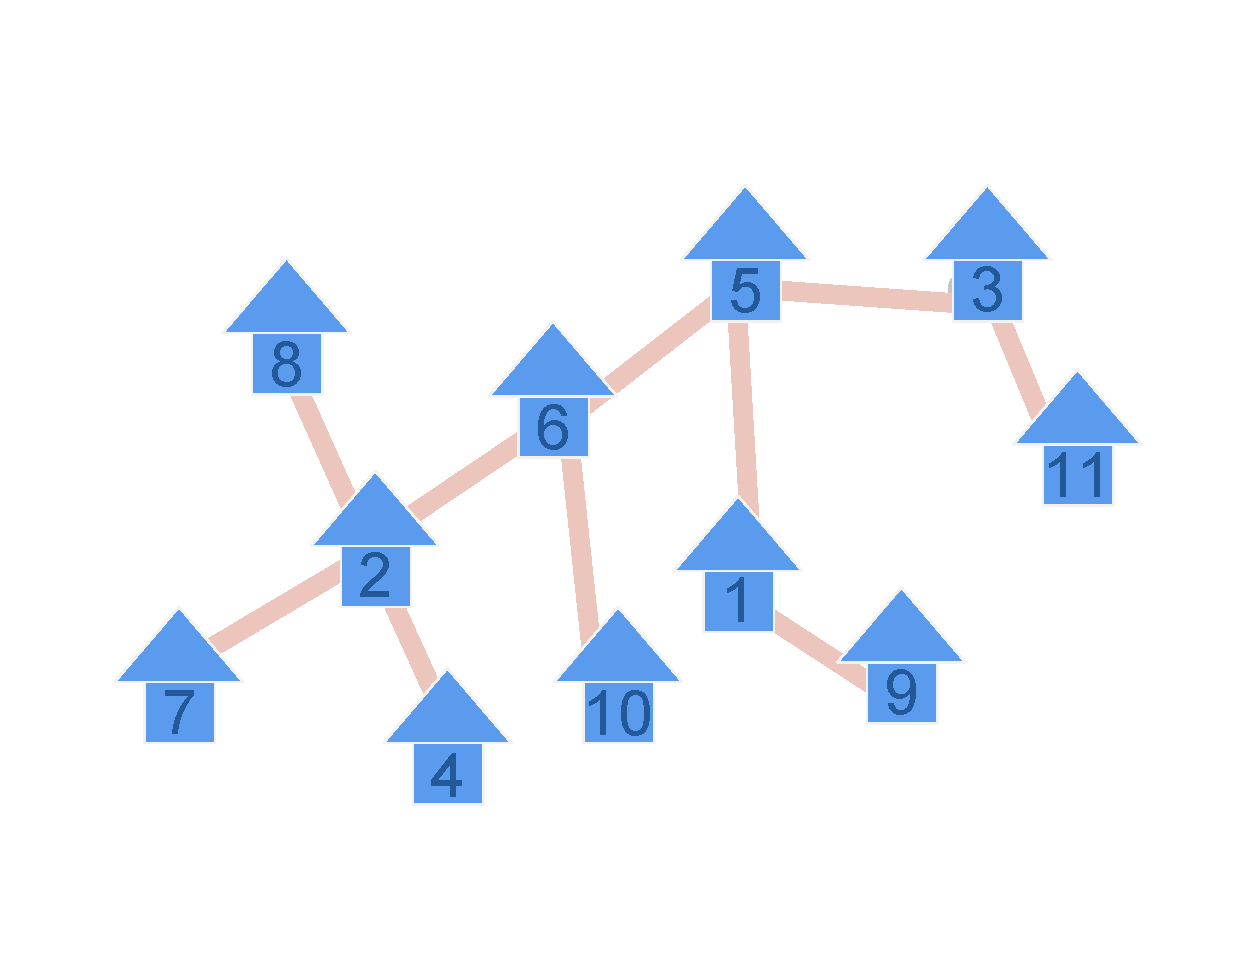
\includegraphics[scale=0.45]{../img/1_infinite_loop__cropped.pdf}
  \caption{\figtabsize {\residenceblock} street map.}
  \label{fig:streetmap}

  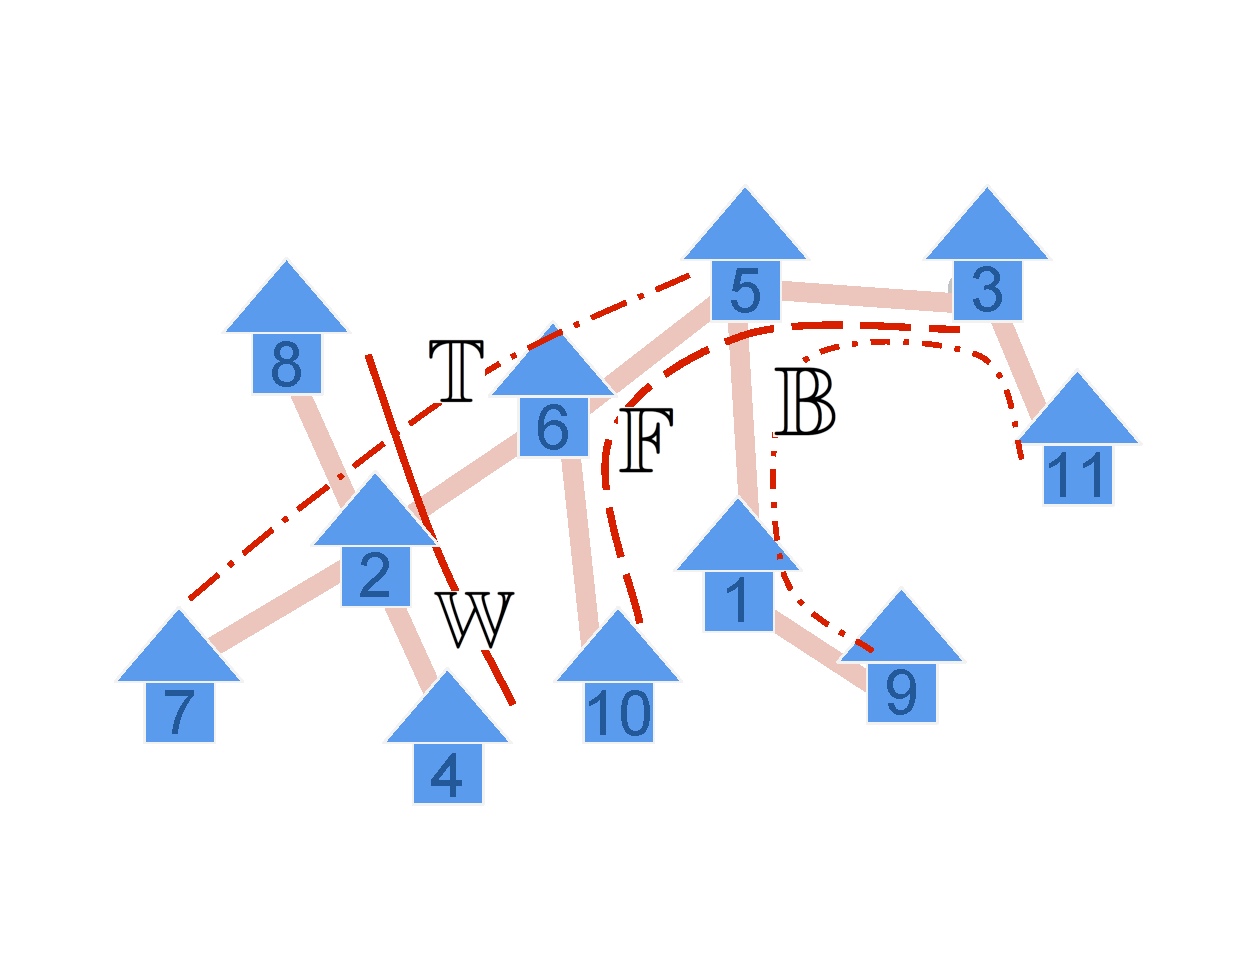
\includegraphics[scale=0.45]{../img/2_infinite_loop_BTWF__cropped.pdf}
  \caption[\figtabsize \residenceblock street map with study group
    routes allocated.]{\figtabsize {\residenceblock} street map with study group
    routes allocated. % Routes are color coded as follows: red for
%     \textcolor{red}{$\xLLL$} group, blue for \textcolor{blue}{$\xGGG$}
%     group, orange for \textcolor{yellow}{$\xBBB$} group, green for
%     \textcolor{green}{$\xTTT$} group
  }
  \label{fig:streetmappath}

  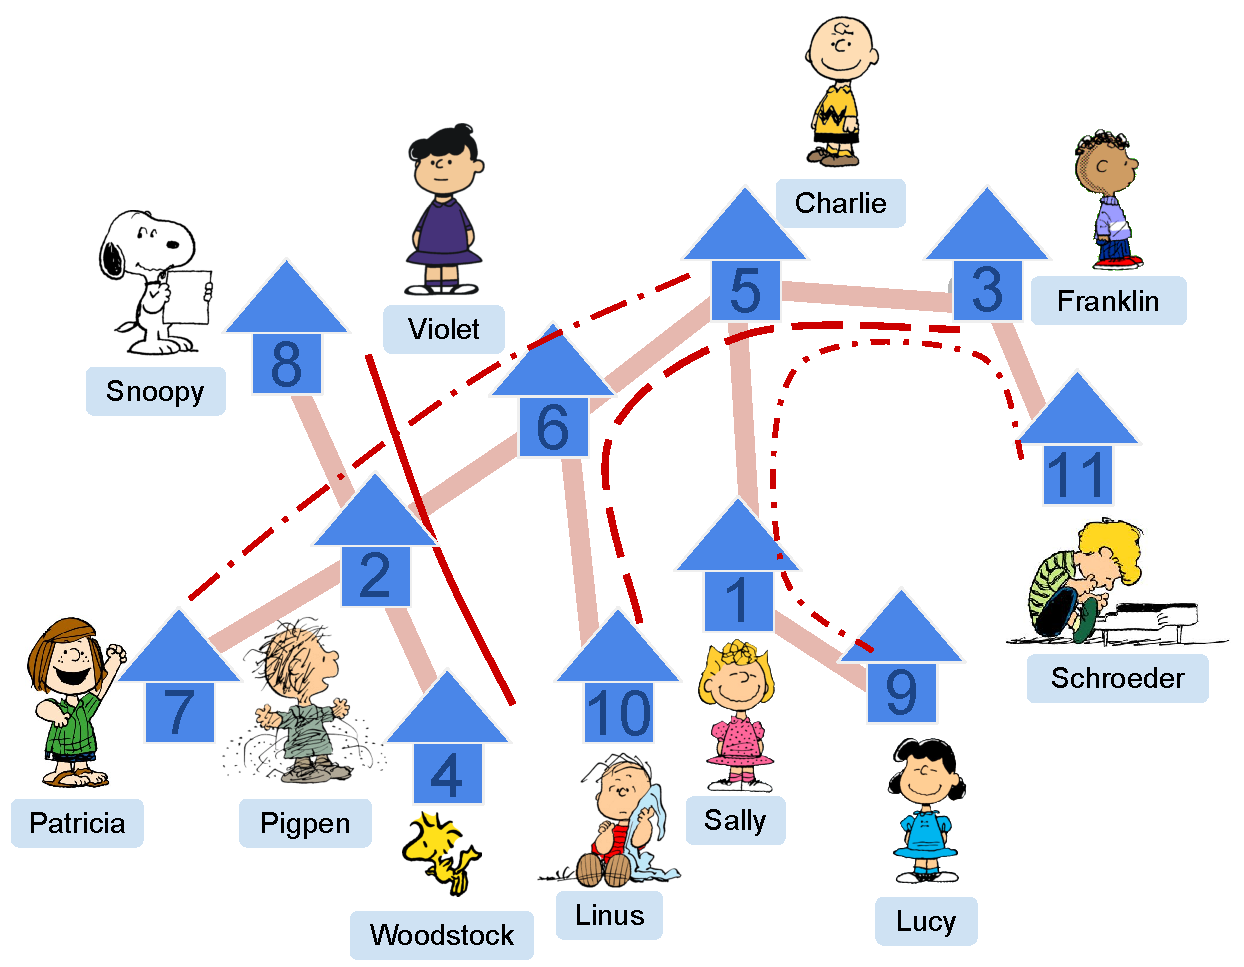
\includegraphics[scale=0.5]{../img/3_infinite_loop.pdf}
  \caption[\figtabsize Solution to the student accommodation
  problem.]{\figtabsize Individual allocation of apartments to
    students in {\residenceblock} that meets the requirements stated
    before.  % The routes are color coded as follows: red for
%     \textcolor{red}{$\xLLL$} group, blue for \textcolor{blue}{$\xGGG$}
%     group, orange for \textcolor{yellow}{$\xBBB$} group, green for
%     \textcolor{green}{$\xTTT$} group.
    \\ {\tiny {\em Peanuts images
        {\copyright} Charles Schulz}}}% YellowOrange
  \label{fig:streetmappathpeople}
\end{figure}

\subsection{Special case}
\label{sec:courseschedule}
As a special case of the study group accommodation problem, suppose
all the apartments are on the same street or if they are all lined up
on a single path, the street map becomes a tree that is just a
path. Then the problem becomes what is called an {\em interval
  assignment problem}. The idea of interval assignment may not be
obvious here; hence to see this, consider a different problem in
{\WSI} where the classes for these study groups courses need to be
scheduled during a day (or a week or any time period). Each study
group has a bunch of courses associated with it some of which may be
shared by two or more study groups. It is mandatory that a student who
is a member of a study group takes all the courses associated with
that group. There are slots during the day for classes to be held and
the problem is to allocate class slots to courses such that all the
classes of a study group are consecutive. % \footnote{It is debatable if this will
% not hamper the attention span and memory retention rate of the
% students but that is undoubtedly out of the scope of this
% thesis.}
The parallels between this class allocation problem and the
accommodation problem can be seen as follows. The set $U$ here, are
the courses offered (say Course 101 {\coneohone}, Course 102
{\coneohtwo} and so on). In this variation of the problem, the
collection $\cF$ is the set of study groups but the study groups are
filled by course IDs (in place of students in the earlier
example). For instance, Course 101 is mandatory for all study groups
$\xLLL$, $\xGGG$, $\xBBB$, $\xTTT$ and Course 102 is mandatory for
only the $\xLLL$ group) and so on. The sequence of class slots for the
day (or week or any time period) is analogous to the street map in the
accommodation problem. It is quite obvious now why this version of the
problem (where the ``target graph'' is a path and not any
tree) is called an interval assignment
problem.

The interval assignment problem to a set system is equivalent to the
consecutive-ones property (COP) problem in binary matrices\cite{wlh02,
  nsnrs09}.  The COP problem is to rearrange rows (columns) of a
binary matrix in such a way that every column (row) has its {\un}s
occur consecutively. If this is possible the matrix is said to have
the COP.  COP is a well researched combinatorial problem and has
several positive results on tests for it and computing the COP
permutation (i.e. the course schedule in the above illustration) which
will be surveyed later in this document. Hence we are interested in
extensions of COP, more specifically, the extension of interval
assignment problem to tree path assignment problem (which is
illustrated by the study group accommodation problem).


\section[Basic preliminaries]{Basic preliminaries} 
\label{sec:basicprelim}

Here we see some basic definitions and conventions necessary for the contents
of this thesis.

\subsection{Matrices}
If $n$ is a positive integer, $[n]$ denotes the set $\{1,2,... n\}$.

\begin{definition}[Binary matrix]
  \label{def:binmatrix}
  Let $M$ be an $n \times m$ matrix. $m_{i,j}$ denotes its $(i,j)$th
  element, i.e. element at $i$th row and $j$th column. $M$ is a
  \textbf{binary matrix} if each of its element is 0 or \un; for all
  $i \in [n]$ and $j \in [m]$, $m_{i,j} \in \{0, \un\}$
\end{definition}

\begin{definition}[Permutation]
  A \textbf{permutation} $\lambda$ of a set $X = \{x_1, x_2, \ldots
  x_n\}$ is a bijection $\lambda: X \rightarrow X$.  $\lambda$ may be
  written as a sequence $x_{i_1}x_{i_2}\ldots x_{i_n}$, where $i_j \in
  [n]$ to mean that $\lambda(x_j)= x_{i_j}$.  This document uses both
  notations as convenient in context.
\end{definition}

The idea of \cop of binary matrices was mentioned a few times in
earlier sections. Now we will see the formal definition of \COP in
Definition~\ref{{def:copmatrix}}.

\begin{definition}[\Cop (on columns)]
  \label{def:copmatrix}
  Let $M$ be a binary matrix.
  \begin{enumerate}
  \hangindent \defindent
  \item A \textbf{block of \un s (block of 0s)} in a column of $M$ is a maximal set of
    consecutive \un-entries (0-entries) in this column.
  \item $M$ has the \textbf{strong \cop
      (strong \COP)} if in every column the \un s appear consecutively,
    \ie if every column contains at most one block of \un s.
  \item $M$ has the \textbf{\cop} if its rows can be
    permuted in such a way that the resulting matrix has the strong \COP.
  \item If an ordering for the rows of $M$ gives the strong \COP, it
    is called a \textbf{\COP order} or \textbf{\COP permutation}.
  \end{enumerate}
\end{definition}

When the roles of rows and columns are exchanged in
Definition~\ref{def:copmatrix}, it defines \COP on rows. Both
are equivalent properties (for the purposes of this thesis) and both
conventions are seen the literature.
Figure~\ref{fig:cop-matrix} gives an example of \COP on columns.

\figcopmatrix

A less restrictive property of binary matrices that is a
generalization of the \COP is \crop (\CROP). The matrix can be
visualized to be wrapped around a horizontal cylinder and demands that
after some row permutations, if required, in every column the \un s
appear consecutively on the cylinder -- note that this implies the 0s
also appear consecutively.

\begin{definition}[\Crop (on columns)]
  \label{def:cropmatrix}
  Let $M$ be a binary matrix.
  \begin{enumerate}
  \hangindent \defindent
  \item $M$ has the \textbf{strong \crop (strong \CROP)} if in every
    column the \un s appear consecutively or the 0s appear
    consecutively or both.
  \item $M$ has the \textbf{\crop (\CROP)} if its rows can be permuted
    in such a way that the resulting matrix has the strong \CROP.
  \item If an ordering for the rows of $M$ gives the strong \CROP,
    then it is called the \textbf{\CROP ordering} or \textbf{\CROP
      permutation}.
  \end{enumerate}
\end{definition}

\subsection{Sets}

\begin{definition}[Set system]
  \label{def:setsystem}
  Let $U$ be a universe with $|U| = n$.  
  \begin{enumerate}
  \hangindent \defindent
  \item The set $\F \subseteq (2^{U} \setminus \emptyset)$ is called a
    \textbf{set system} with universe $U$.
  \item Two sets $S, S' \in \cF$ are said to \textbf{overlap}, denoted
    by $S \overlap S'$, if they have a non-empty intersection and
    neither is contained in the other.
    \[S \overlap S' \text{ \iff\ } S \cap S' \ne \emptyset, S
    \nsubseteq S', S' \nsubseteq S\]
  \end{enumerate}
\end{definition}


\begin{definition}
  \label{def:poset}    
%   Let $A$ be a set and $R$ be a binary relation $R \subseteq A \times
%   A$.

%   \textbf{poset}
  Let $X$ be a partially ordered set with $\preccurlyeq$ being the
  partial order on $X$.

  \begin{enumerate}
  \hangindent \defindent
%  \item \textbf{hasse diagram}
  \item An element $X_m \in X$ is a
    \textbf{maximal upper bound} of $X$ if $\nexists X_q \in X$ such
    that $X_m \preccurlyeq X_q$.  A maximal upper bound on $X$ is
    denoted by $mub(X)$.

  \item A set of sets form a \textbf{single
      inclusion chain} when the Hasse diagram of their subset relation
    forms a single chain.
  \end{enumerate}
\end{definition}

\subsection{Graphs}

\begin{definition}[Graph, Tree, Path]
  \label{def:graphtree}
  \begin{enumerate}
    \hangindent \defindent
  \item An \textbf{(undirected) graph} is $G = (V,E)$ is \stt $V$ is a
    finite set and $E$ is a set of ordered pairs, $E \subseteq V
    \times V$. An element in $V$ is called a \textbf{vertex
      (\emph{pl.} vertices)} and an element from $E$ is called an
    \textbf{edge}. $V$ and $E$ may be written as $V(G)$ and $E(G)$
    respectively. If $u,v \in V$ and $(u,v) \in E$ then $v$ is said to
    be \textbf{adjacent} to $u$ and vice versa. A \textbf{subgraph} of
    $G$ is a graph $G' = (V',E')$ \stt $V' \subseteq V$ and $E'
    \subseteq E$.

  \item A \textbf{path} is a graph $P = (V,E)$ with vertex set $V =
    \{v_1,\ldots,v_n\}$ and edge set $E= \{ (v_1,v_2),(v_2,v_3),
    \ldots,(v_{n-2},v_{n-1}),(v_{n-1},v_{n})\}$. The vertices $v_1,
    v_n$ are called the \textbf{endpoints} of $P$. The graph $P$ is
    called a \textbf{cycle} if it has an additional edge $(v_n,v_1)$.

  \item A \textbf{tree} is a graph $T$ that has no subgraph that is a
    cycle.
  \end{enumerate}
\end{definition}

% When refering to a tree as $T$ it could be a reference to the tree
% itself, or the vertices of the tree. This will be clear from the
% context.

\begin{definition}[Intersection graph]
  \label{def:intersectiongraph}
  Let $\cF$ be a set system. Then its \textbf{intersection graph}
  $\bI(\cF)$ is a graph \stt its vertex set has a bijection to $\cF$
  and there exists an edge between two vertices \iff their
  corresponding sets in $\cF$ have a non-empty intersection.
\end{definition}

\begin{definition}[Interval graph, Path graph]
  \label{def:pathgraph}
  Let $G$ be a graph.
  \begin{enumerate}
  \hangindent \defindent
  \item $G$ is an \textbf{interval graph} if there a set of intervals
    $\cI$ \stt $G$ is isomorphic to the intersection graph of
    $\cI$. \[G \cong \bI(\cI)\]
  \item $G$ is a \textbf{path graph} if there exists a tree $T$ and a
    set of paths from $T$, $\cP$ \stt $G$ is isomorphic to the
    intersection graph of $\cP$. \[G \cong \bI(\cP)\]
  \item $G$ is a \textbf{chordal graph} if it has no induced cycle of
    length greater than 3. Moreover, a \textbf{chordal graph} is
    characterized as an intersection graph of subtrees of a tree.
  \end{enumerate}
\end{definition}



\section[Brief Survey]{Consecutive-ones Property - a Brief Survey}
\label{sec:background}

In this section, a brief survey of the consecutive-ones problem and
its optimization problems is presented.


\subsection{Matrices with COP}
\label{sec:copmatrices}
As seen earlier, the interval assignment problem (illustrated as the
course scheduling problem in Section~\ref{sec:problem}), is a special
case of the problem we address in this thesis, namely the tree path
labeling problem (illustrated as the \illustrationproblem). The
interval assignment problem and COP problem are equivalent
problems. In this section we will see some of the results that exists
in the literature today towards solving the COP problem and
optimization problems surrounding it.

% \begin{figure}[t] %[htbp]
%   \centering

%   {\figtabsize
%     \begin{tabular}[h]{l|lcccl}
%       $M_1$: & $M_1'$: &&&& $M_2$:\\
%       &&&&&\\
%       \begin{tabular}[h]{llll}
%         $c_1$ & $c_2$ &$c_3$ &$c_4$\\
%         &&&\\
%         \un & 0   & \un & 0\\
%         0   & \un & 0   & \un \\
%         \un & 0   & 0   & \un
%       \end{tabular}
%       &
%       \begin{tabular}[h]{llll}
%         $c_3$ &$c_1$ &$c_4$& $c_2$\\
%         &&&\\
%         \un & \un & 0 & 0\\
%         0 & 0 & \un & \un \\
%         0 & \un & \un & 0
%       \end{tabular}
%       &&&&
%       \begin{tabular}[h]{llll}
%         $d_1$ & $d_2$ &$d_3$ &$d_4$\\
%         % &&&\\
%         &&&\\
%         \un & \un & 0 & 0\\
%         0 & \un & \un & 0 \\
%         0 & \un & 0 & \un 
%       \end{tabular}
%     \end{tabular}
%   }

%   \caption[\figtabsize Matrices with and without COP.]{\figtabsize
%     Matrices with and without COP. $M_1$ has COP because by permuting
%     its columns, $c_1$-$c_4$, one can obtain $M_1'$ where the {\un}s
%     in each row are consecutive. $M_2$, however, does not have COP
%     since no permutation of its columns, $d_1$-$d_4$, will arrange
%     {\un}s in each row consecutively \cite{d08phd}.}

%   \label{fig:cop-matrix}
% \end{figure}

Recall that a matrix with COP is one whose rows (columns) can be
rearranged so that the {\un}s in every column (row) are in consecutive
rows (columns). % Figure~\ref{fig:cop-matrix} shows examples of this
% property. 
COP in binary matrices has several practical applications
in diverse fields including scheduling \cite{hl06}, information
retrieval \cite{k77} and computational biology \cite{abh98}.  Further,
it is a tool in graph theory \cite{mcg04} for interval graph
recognition, characterization of Hamiltonian graphs, planarity testing
\cite{bl76} and in integer linear programming \cite{ht02,hl06}.


The obvious first questions after being introduced to the consecutive
ones property of binary matrices are if COP can be detected
efficiently in a binary matrix and if so, can the COP permutation of
the matrix also be computed efficiently?  Recognition of COP in a
binary matrix is polynomial time solvable and the first such algorithm
was given by \cite{fg65}.  A landmark result came a few years later
when \cite{at72} discovered the families of forbidden submatrices that
prevent a matrix from having COP and most, if not all, results that
came later were based on this discovery which connected COP in binary
matrices to convex bipartite graphs. In fact, the forbidden
submatrices came as a corollary to the discovery that convex bipartite
graphs are AT-free on at least one of the partitions in
\cite{at72}. The first linear time algorithm for COP testing (COT) was
invented by \cite{bl76} using a data structure called \PQtrees.  Since
then several COT algorithms have been invented -- some of which
involved variations of \PQtrees \cite{mm96,wlh01,mcc04}, some involved
set theory and ICPIA \cite{wlh02,nsnrs09}, parallel COT
algorithms\cite{as95,bs03,ly91} and certifying algorithms\cite{mcc04}.

The construction of \PQtrees in \cite{bl76} draws on the close
relationship of matrices with \COP to interval graphs. A PQ tree of a
matrix is one that stores all row (column) permutations of the matrix
that give the COP orders (there could be multiple orders of rows or
columns) of the matrix. This is constructed using an elaborate linear
time procedure and is also a test for planarity.  PQR trees is a
generalized data structure based on PQ trees \cite{mm96,mpt98}.
\cite{tm05} describes an improved algorithm to build PQR
trees. \cite{wlh02} describes the simpler algorithm for COT. Hsu also
invented PC trees \cite{wlh01} which is claimed to be much easier to
implement. \cite{nsnrs09} describes a characterization of
consecutive-ones property solely based on the cardinality properties
of the set representations of the columns (rows); every column (row)
is equivalent to a set that has the row (column) indices of the rows
(columns) that have one entries in this column (row). This is
interesting and relevant, especially to this thesis because it
simplifies COT to a great degree.

\cite{mcc04} describes a different approach to COT. While all previous
COT algorithms gave the COP order if the matrix has the property but
exited stating negative if otherwise, this algorithm gives an evidence
by way of a certificate of matrix even when it has no COP. This
enables a user to verify the algorithm's result even when the answer
is negative. This is significant from an implementation perspective
because automated program verification is hard and manual verification
is more viable. Hence having a certificate reinforces an
implementation's credibility. Note that when the matrix {\em has} COP,
the COP order is the certificate.  The internal machinery of this
algorithm is related to the weighted betweenness problem
addressed in \cite{co98}.  

\subsection{Optimization problems in COP}
\label{sec:optcop}

So far we have been concerned about matrices that have the consecutive
ones property. However in real life applications, it is rare that data
sets represented by binary matrices have COP, primarily due to the
noisy nature of data available. At the same time, COP is not arbitrary
and is a desirable property in practical data representation
\cite{co98,jkckv04,k77}. In this context, there are several
interesting problems when a matrix does not have COP but is ``close''
to having COP or is allowed to be altered to have COP. These are the
optimization problems related to a matrix which does not have
COP. Some of the significant problems are surveyed in this section.

\cite{at72} showed that a matrix that does not have COP have certain
substructures that prevent it from having COP. Tucker classified these
forbidden substructures into five classes of submatrices. This result
is presented in the context of convex bipartite graphs which
\cite{at72} proved to be AT-free in one of the partitions. By
definition, convex bipartite graph have half adjacency matrices that
have COP on either rows or columns (graph is biconvex if it has COP on
both)\cite{d08phd}. A half adjacency matrix is a binary matrix
representing a bipartite graph as follows. The set of rows and the set
of columns form the two partitions of the graph. Each row node is
adjacent to those nodes that represent the columns that have {\un}s in
the corresponding row. \cite{at72} proves that this bipartite graph
has no asteroidal triple in vertex partition corresponding to rows if
and only if the matrix has COP on columns and goes on to identify the
forbidden substructures for these bipartite graphs. The matrices
corresponding to these substructures are the forbidden submatrices.

Once a matrix has been detected to not have COP (using any of the COT
algorithms mentioned earlier), it is naturally of interest to find out
the smallest forbidden substructure (in terms of number of rows and/or
columns and/or number of entries that are {\un}s). \cite{d08phd}
discusses a couple of algorithms which are efficient if the number of
{\un}s in a row is small. This is of significance in the case of
sparse matrices where this number is much lesser than the number of
columns. $(*,\Delta)${\em -matrices} are matrices with no restriction
on number of {\un}s in any column but have at most $\Delta$ {\un}s in
any row. {\sc Min COS-R (Min COS-C), Max COS-R (Max COS-C)} are
similar problems which deals with inducing COP on a matrix. In {\sc
  Min COS-R (Min COS-C)} the question is to find the minimum number of
rows (columns) that must be deleted to result in a matrix with COP.
In the dual problem {\sc Max COS-R (Max COS-C)} the search is for the
maximum number of rows (columns) that induces a submatrix with
COP. Given a matrix $M$ with no COP, \cite{b75-phd} shows that finding
a submatrix $M'$ with all columns\temptext{ check if b75 deals with
  COP col or COP row. also is it any submatrix with k less than r rows
  or submatrix must have all columns? } but a maximum cardinality
subset of rows such that $M'$ has COP is NP complete. \cite{hg02}
corrects an error of the abridged proof of this reduction as given in
\cite{gj79}.  \cite{d08phd} discusses all these problems in detail
giving an extensive survey of the previously existing results which
are almost exhaustively all approximation results and hardness
results. Taking this further, \cite{d08phd} presents new results in
the area of parameterized algorithms for this
problem.

Another problem is to find the minimum number of entries in the matrix
that can be toggled to result in a matrix with COP.  \cite{v85}
discusses approximation of {\sc COP Augmentation} which is the problem
of changing of the minimum number of zero entries to {\un}s so that
the resulting matrix has COP. As mentioned earlier, this problem is
known to be NP complete due to \cite{b75-phd}. \cite{v85} also proves,
using a reduction to the longest path problem, \temptext{ or is it a
  survey of another result?  check.} that finding a Tucker's forbidden
submatrix of at least $k$ rows is NP complete. \temptext{ how is this
  different from booth's 75 result??}  

\cite{jkckv04} discusses the use of matrices with almost-COP (instead
of one block of consecutive {\un}s, they have $x$ blocks, or {\em
  runs}, of consecutive {\un}s and $x$ is not too large) in the
storage of very large databases.  The problem is that of reordering of
a binary matrix such that the resulting matrix has at most $k$ runs of
{\un}s. This is proved to be NP hard using a reduction from the
Hamiltonian path problem.


% \section[Some applications of \COP]{Application of COP in Areas of Graph Theory and
%   Algorithms}
% \label{sec:appcopGTA}

% \temptext{Combine COP in Relational Database Model + COP in Graph
%   Isomorphism + Certifying Algorithms}

% %\subsection{COP in Relational Database Model}
% \label{sec:apprdbm}
% \tnote{(set systems theme)}

% %\subsection{}
% \label{sec:appgraphiso}
% \tnote{(canonization theme)}

% %\subsection{}
% \label{sec:appcertalgo}
% \tnote{ (certification McC04 theme)}


\section[Generalization of COP]{Generalization of COP - the Motivation}
\label{sec:motive}
Section~\ref{sec:copmatrices} introduced a succinct characterization
for consecutive-ones property which is solely based on the cardinality
properties of the set representations of the matrix's columns
\cite{nsnrs09}. This result is very relevant to this thesis because
aside from it simplifying COT to a great degree, our generalization
problem is motivated by their results.

\cite{nsnrs09} characterizes interval assignments to the sets which
can be obtained from a single permutation of the rows.  For an
assignment to be feasible, the cardinality of the interval assigned to
each set in the system must be same as the cardinality of the set, and
the intersection cardinality of any two intervals must be same as the
intersection cardinality of their corresponding sets.  While this is
obviously a necessary condition, this result shows this is also
sufficient.  \cite{nsnrs09} calls this an Intersection Cardinality
Preserving Interval Assignment (ICPIA).  This paper generalizes the
idea from \cite{wlh02} of decomposing a given binary matrix into prime
matrices for COT and describes an algorithm to test if an ICPIA exists
for a given set system.

The equivalence of the problem of testing for the consecutive-ones
property to the constraint statisfaction problem of interval
assignment \cite{nsnrs09} or interval labeling \cite{kklv10} is as
follows. Every column (row) of the binary matrix can be converted into
a set of non-negative integers which are the indices of rows (columns)
with {\un}s in that column (row). It is apparent that if the matrix
has COP in columns (rows), then constructing such sets after applying
the COP permutation to the rows (columns) of the matrix will result in
sets with consecutive integers. In other words, after application of
COP reordering, the sets are intervals. Indeed the problem now becomes
finding interval assignments to a given set system such that there
exists a permutation of the universe of set of row indices (column
indices) which converts each set to its assigned interval.

The problem of interest in this thesis, namely, tree path labeling
problem, is a natural generalization of the interval assignment
problem or the COT problem. The problem is defined as follows -- given
a set system $\cF$ from a universe $U$ and a target tree $T$, does
there exist a bijection from $U$ to the vertices of $T$ such that each
set in the system maps to a path in $T$.  We refer to this as the
{\CFTPL} problem or simply {\em tree path labeling} problem for an
input set system and target tree pair -- $(\cF,T)$. The special case
of the target tree being a path, is the interval assignment problem.
We focus on generalizing the notion of an ICPIA \cite{nsnrs09} to
characterize feasible path assignments.  We show that for a given set
system $\cF$, a tree $T$, and an assignment of paths from $T$ to the
sets, there is a feasible\footnote{The notion of {\em feasibility} is
  formally defined in Section~\ref{ch:prelims}.}  bijection between
$U$ and $V(T)$ if and only if the intersection cardinalities among any
three sets (not necessarily distinct) is equal to that of the
corresponding paths assigned to them and the input passes a filtering
algorithm (described in this paper) successfully.  This algorithmic
characterization gives a natural data structure that stores all the
\remove{relevant} feasible bijections between $U$ and $V(T)$. This
reduces the search space for the solution considerably from the
universe of all possible bijections between $U$ and $V(T)$ to only
those bijections that maintain the characterization.  Further, the
filtering algorithm is also an efficient algorithm to test if a tree
path labeling\footnote{The terms {\em tree path labeling} and {\em
    tree path assignment} are, in informal language,
  synonyms. Formally, the former refers to the bijection $\cl: \cF
  \rightarrow \cP$. The latter refers to the set of ordered pairs
  $\{(S, P) \mid S \in \cF, P \in \cP\}$. $\cP$ is a set of paths on
  $T$.} is feasible.


\section[Summary of new results]{Summary of New Results in this Thesis}
\label{sec:results}

We see in Section~\ref{sec:motive} that pairwise intersection
cardinality preservation is necessary and sufficient for an interval
assignment to be feasible for a given hypergraph\footnote{A {\em
    hypergraph} is an alternate representation of a set system and
  will be used in this thesis.}~\footnote{See Section~\ref{ch:prelims}
  for the formal definition.} and thus is a characterization for COP
\cite{nsnrs09}. In our work we extend this characterization and find
that trio-wise intersection cardinality preservation makes a tree path
labeling\footnote{A {\em tree path labeling} $\cl$ is a bijection of
  paths from the target tree $T$ to the hyperedges in given hypergraph
  $\cF$.}~\footnotemark[4] (TPL) feasible, which is a generalization
of the COP problem. This problem is defined by \FTPL (See
Section~\ref{sec:myresearchintro} for problem definition). %as follows.

% {\small
%   \begin{minipage}[h]{5in}
%     % \begin{singlespace}
%     \vspace{2mm}
%     {\large \FTPL}\\
%     \begin{tabular}[t]{l|l}
%       \hline\\
%       {\tt Input} & 
%       \begin{minipage}[t]{\probdefwidth}
%         A hypergraph $\cF$ with vertex set $U$, a tree $T$, a set of
%         paths $\cP$ from $T$ and a
%         bijection $\cl$~$:$~$\cF \rightarrow \cP$.\\
%       \end{minipage}\\
%       {\tt Question} &
%       \begin{minipage}[t]{\probdefwidth}
%         Does there exist a bijection $\phi$~$:$~$U \rightarrow V(T)$
%         such that $\phi$ when applied on any hyperedge in $\cF$ will
%         give
%         the path mapped to it by the given tree path labeling $\cl$.\\
%         { i.e., $\cl(S) = \{\phi(x) \mid x \in S\}$, for every
%           hyperedge $S \in \cF$.}
%       \end{minipage}\\
%     \end{tabular}
%     % \end{singlespace}
%   \end{minipage}\\
% }

We give a necessary and sufficient condition by way of {\em
  Intersection Cardinality Preservation Path Labeling} (ICPPL) and a
filtering algorithm for {\FTPL} to output in affirmative. ICPPL
captures the trio-wise cardinality property described
earlier\footnote{See Section~\ref{sec:feasible} for the definition of
  ICPPL.}. This characterization can be checked in polynomial time.  A
relevant consequence of this constructive procedure is that it is
sufficient to iteratively check if three-way intersection
cardinalities are preserved.  In other words, in each iteration, it is
sufficient to check if the intersection of any three hyperedges is of
the same cardinality as the intersection of the corresponding paths.
Thus this generalizes the well studied question of the feasible
interval assignment problem which is the special case when the target
tree $T$ is simply a path \cite{wlh02,nsnrs09}.

Aside from checking if a given TPL is feasible, we also solve the
problem of computing a feasible TPL for a given hypergraph and target
tree, if one exists. This problem is the {\CFTPL} problem (See
Section~\ref{sec:myresearchintro} for problem definition). %, is defined as follows.

% {\small
%   \begin{minipage}[h]{5in}
%     % \begin{singlespace}
%     \vspace{2mm}
%     {\large \CFTPL}\\
%     \begin{tabular}[t]{l|l}
%       \hline\\
%       {\tt Input} & 
%       \begin{minipage}[t]{\probdefwidth}
%         A hypergraph $\cF$ with vertex set $U$ and a tree $T$.\\
%       \end{minipage}\\

%       {\tt Question} &
%       \begin{minipage}[t]{\probdefwidth}
%         Does there exist a set of paths $\cP$ from $T$ and a bijection
%         $\cl$~$:$~$\cF \rightarrow \cP$, such that {\FTPL} returns
%         {\bf true} on $(\cF, T, \cl)$.
%       \end{minipage}\\
%     \end{tabular}
%     % \end{singlespace}
%   \end{minipage}\\
% }

We present a polynomial time algorithm for {\CFTPL} when the target
tree $T$ belongs to a special class of trees called {\em \kstars} and
when the hyperedges in the hypergraph $\cF$ have at most $k+2$
vertices (\CFTPLKTREE -- See Section~\ref{sec:myresearchintro} for
problem definition). A couple of examples of {\kstars} are given in
Figure~\ref{fig:ksubstar}.


\begin{figure}[t]
  \centering
  \begin{tabular}[h]{ccccc}
    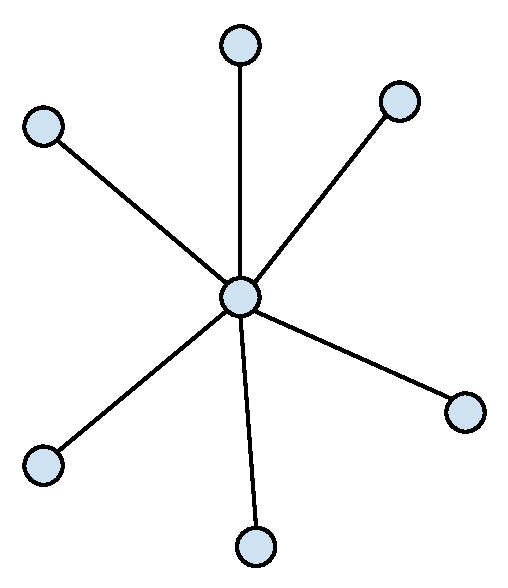
\includegraphics[scale=0.3]{../img/star.pdf} &&&&
    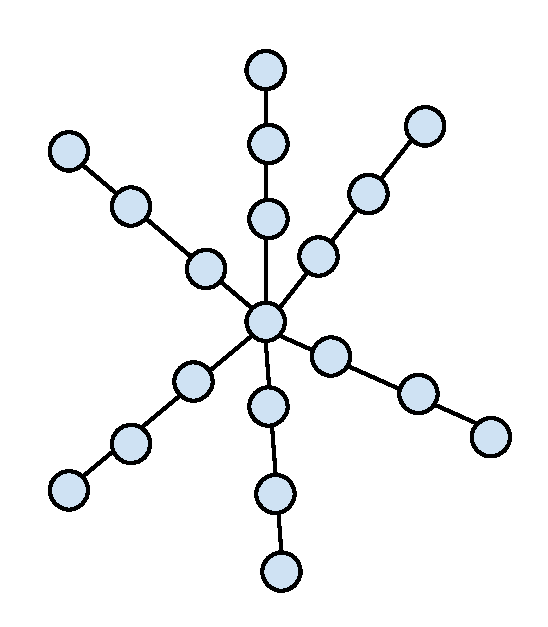
\includegraphics[scale=0.3]{../img/kstar.pdf}\\
    (a) &&&& (b)
  \end{tabular}
  \caption{\figtabsize Examples of {\kstars}. (a) $k = 0$ (b) $k = 2$
  }
  \label{fig:ksubstar}
\end{figure}

% {\small
%   \begin{minipage}[h]{5in}
%     % \begin{singlespace}
%     \vspace{2mm}
%     {\large \CFTPLKTREE}\\
%     \begin{tabular}[t]{l|l}
%       \hline\\
%       {\tt Input} & 
%       \begin{minipage}[t]{\probdefwidth}
%         A hypergraph $\cF$ with vertex set $U$ such that every
%         hyperedge
%         $S \in \cF$ is of cardinality at most $k+2$ and a {\kstar} $T$.\\
%       \end{minipage}\\
%       {\tt Question} &
%       \begin{minipage}[t]{\probdefwidth}
%         Does there exist a set of paths $\cP$ from $T$ and a bijection
%         $\cl$~$:$~$\cF \rightarrow \cP$, such that {\FTPL} returns
%         {\bf true} on $(\cF, T, \cl)$.
%       \end{minipage}\\
%     \end{tabular}
%     % \end{singlespace}
%   \end{minipage}\\
% }

In spite of this being a restricted case, we believe that our results
are of significant interest in understanding the nature of {\sc Graph
  Isomorphism} which is polynomial time solvable in interval graphs
while being hard on path graphs\cite{kklv10}. {\kstars} are a class of
trees which are in many ways very close to intervals or paths. Each
ray\footnote{The path from a leaf to the root, the vertex with highest
  degree, is called a {\em ray} of the \kstar.}~\footnotemark[4] are
independent except for the root\footnote{The vertex with maximum
  degree in a {\kstar} is called {\em root}.}~\footnotemark[4] and
hence can be considered as an independent interval till the root. Our
algorithm builds on this fact and uses the interval assignment
algorithm\cite{nsnrs09} up until ``reaching'' the root and then uses
the trio-wise intersection cardinality (the extra condition in ICPPL
that generalizes ICPIA) check to resolve the ambiguity about which ray
the algorithm should ``grow'' the solution into in the next iteration.

We also have an algorithm for solving {\CFTPL} with no restrictions on
the target tree or set size which runs in exponential time.  This
algorithm finds a path labeling from $T$ by decomposing the problem
into subproblems of finding path labeling of subsets of $\cF$ from
subtrees of $T$. Given the fact that binary matrices naturally
represent a set system (see Section~\ref{sec:motive}) and that the
{\em overlap} relation between the sets involved is an obvious
equivalence relation, $\cF$ quite naturally partitions into
equivalence classes known as {\em overlap components}. In the context
of COP, overlap components were used in \cite{wlh02} and
\cite{kklv10}. Moreover, \cite{nsnrs09} discovered that these
equivalence classes form a total order. We extend this to TPL and find
that when $\cF$ is a path hypergraph\footnote{If there exists an FTPL
  for a hypergraph $\cF$, it is called a path hypergraph.}, the
classes can be partially ordered as an in-tree in polynomial
time. Once $\cF$ is ``broken'' into overlap components, one must
identify the subtree of $T$ that it needs to map to and this is the
hard part which is currently open to be solved in polynomial time.
